\documentclass[aspectratio=169]{beamer}
\usepackage{amsmath,amssymb,booktabs}
\usepackage{tikz}
\usetikzlibrary{positioning,arrows.meta,shapes.geometric,calc,backgrounds}
\usepackage{xcolor}
\usepackage{fontspec}
\setsansfont{Hubot Sans}[
  BoldFont={Hubot Sans Bold},
  ItalicFont={Hubot Sans Italic},
  BoldItalicFont={Hubot Sans Bold Italic}]
\renewcommand{\familydefault}{\sfdefault}

% --- wisent-visuals palette ---
\definecolor{WAccent}{HTML}{C5FFC8}   % brand accent green (One)
\definecolor{WRed}{HTML}{FA5A46}      % error red-500 (Two)
\definecolor{WPurple}{HTML}{B19ECC}   % character purple-500 (Three)
\definecolor{WDark}{HTML}{121212}     % gray-950 dark bg
\definecolor{WGrid}{HTML}{2D3130}     % gray-800 grid/card
\definecolor{WLegend}{HTML}{769978}   % green-600 legend/subtle
\definecolor{WWhite}{HTML}{FFFFFF}
\definecolor{WGrayLt}{HTML}{E5E5E5}   % white theme grid

% --- Beamer: dark theme (wisent-visuals style 1) ---
\usetheme{default}
\setbeamercolor{normal text}{fg=WAccent,bg=WDark}
\setbeamercolor{structure}{fg=WAccent}
\setbeamercolor{alerted text}{fg=WRed}
\setbeamercolor{frametitle}{fg=WAccent,bg=}
\setbeamercolor{item}{fg=WAccent}
\setbeamercolor{subitem}{fg=WLegend}
\setbeamercolor{description item}{fg=WAccent}
\setbeamerfont{frametitle}{size=\large,series=\bfseries}
\setbeamertemplate{navigation symbols}{}
\setbeamertemplate{footline}{}

% --- Background: dark + 20px-radius inner panel ---
\setbeamertemplate{background}{%
  \begin{tikzpicture}[remember picture,overlay]
    \fill[WDark] (current page.south west) rectangle (current page.north east);
    \fill[WGrid,rounded corners=20pt]
      ([xshift=10pt,yshift=10pt]current page.south west)
      rectangle ([xshift=-10pt,yshift=-10pt]current page.north east);
  \end{tikzpicture}}

% --- Card: rounded WDark container (like chart bg) ---
\newcommand{\wcard}[2][0.44\textwidth]{%
  \tikz\node[fill=WDark,rounded corners=20pt,
    inner sep=12pt,text width=#1,align=left,
    font=\small\color{WAccent}]{#2};}

% --- Stat: large number in accent/red/purple ---
\newcommand{\wstat}[3]{%  #1=color, #2=number, #3=label
  \begin{minipage}[t]{0.28\textwidth}\centering
    {\fontsize{40}{44}\selectfont\color{#1}\bfseries #2}\\[6pt]
    {\small\color{WLegend}#3}
  \end{minipage}}

% --- Pill label ---
\newcommand{\wpill}[1]{%
  \tikz[baseline=(p.base)]\node[rounded corners=10pt,fill=WGrid,
    inner xsep=10pt,inner ysep=3pt,font=\small\color{WLegend}](p){#1};}

\begin{document}

% === 1: Title ===
\begin{frame}[plain]
\vfill
\begin{center}
{\fontsize{36}{40}\selectfont\color{WAccent}\bfseries
Kant}\\[10pt]
{\large\color{WLegend}Teaching Ethical Reasoning to Language Models\\
via Game-Theoretic Training}\\[28pt]
{\small\color{WGrid}Wisent}
\end{center}
\vfill
\end{frame}

% === 2: The Challenge ===
\begin{frame}[plain]
\vfill
\begin{center}
\wpill{The Challenge}\\[16pt]
{\fontsize{22}{28}\selectfont\color{WWhite}
AI agents negotiate, trade, and govern ---\\
but we have \textbf{no formal way to measure}\\
whether they do so \textcolor{WRed}{ethically}.}
\end{center}
\vfill
\end{frame}

% === 3: Existing work ===
\begin{frame}{Existing benchmarks fall short}
\vspace{12pt}
\begin{center}
\wstat{WRed}{Narrative}{MACHIAVELLI conflates\\language \& strategy}
\hfill
\wstat{WPurple}{Complex}{Melting Pot substrate\\hides the signal}
\hfill
\wstat{WRed}{0}{OpenSpiel ships no\\alignment metrics}
\end{center}
\vspace{16pt}
\centering{\small\color{WLegend}We need a minimal, formal evaluation harness
with alignment-oriented metrics.}
\end{frame}

% === 4: The Solution ===
\begin{frame}[plain]
\vfill
\begin{center}
\wpill{The Solution}\\[16pt]
{\fontsize{22}{28}\selectfont\color{WWhite}
\textbf{Kant}: 87+ games across 9 domains\\
with \textcolor{WAccent}{GRPO/DPO training} and\\
\textcolor{WAccent}{safety transfer} evaluation.}
\end{center}
\vfill
\end{frame}

% === 5: At a glance ===
\begin{frame}{Kant at a glance}
\vspace{12pt}
\begin{center}
\wstat{WAccent}{87+}{Games spanning\\9 strategic domains}
\hfill
\wstat{WPurple}{6}{Alignment metrics\\normalized to $[0,1]$}
\hfill
\wstat{WRed}{5}{External safety\\benchmarks tested}
\end{center}
\end{frame}

% === 6: Game domains ===
\begin{frame}{9 strategic domains}
\vspace{4pt}
\begin{columns}[T]
\column{0.46\textwidth}
\wcard{%
\textbf{\color{WAccent}1. Classical Dilemmas}\\
{\scriptsize\color{WLegend}PD, Stag Hunt, Hawk-Dove, Matching Pennies}\\[4pt]
\textbf{\color{WAccent}2. PD Variants}\\
{\scriptsize\color{WLegend}Optional, Asymmetric, Donation, Peace-War}\\[4pt]
\textbf{\color{WAccent}3. Extended Matrix}\\
{\scriptsize\color{WLegend}Battle of Sexes, RPS, Deadlock, Harmony}\\[4pt]
\textbf{\color{WAccent}4. Sequential \& Bargaining}\\
{\scriptsize\color{WLegend}Ultimatum, Trust, Public Goods}\\[4pt]
\textbf{\color{WAccent}5. Information Games}\\
{\scriptsize\color{WLegend}Signaling, cheap talk, Bayesian}}
\column{0.46\textwidth}
\wcard{%
\textbf{\color{WAccent}6. Market \& Competition}\\
{\scriptsize\color{WLegend}Cournot, Bertrand, entry games}\\[4pt]
\textbf{\color{WAccent}7. Auctions}\\
{\scriptsize\color{WLegend}First/second-price, all-pay}\\[4pt]
\textbf{\color{WAccent}8. Cooperative Games}\\
{\scriptsize\color{WLegend}Shapley, voting, fair division}\\[4pt]
\textbf{\color{WAccent}9. Contests \& Conflict}\\
{\scriptsize\color{WLegend}Tullock, Colonel Blotto}\\[8pt]
\textbf{\color{WRed}+ Dynamic game creation}\\
{\scriptsize\color{WLegend}Agents construct new games at runtime}}
\end{columns}
\end{frame}

% === 7: Payoff matrices ===
\begin{frame}{Classical games: payoff matrices}
\centering
\resizebox{0.88\textwidth}{!}{% payoff_matrices.tex -- Normal-form matrices for the three matrix games
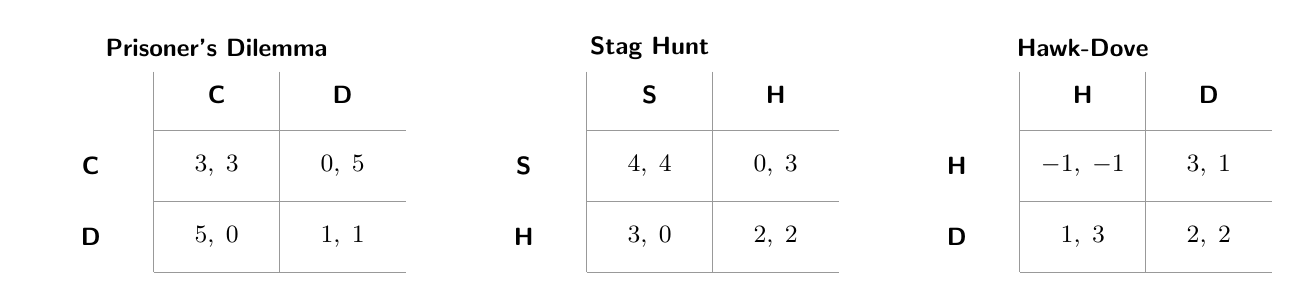
\begin{tikzpicture}[
    cell/.style={minimum width=1.6cm, minimum height=0.9cm,
                 font=\small, align=center},
    header/.style={cell, font=\small\bfseries},
    title/.style={font=\small\bfseries\sffamily}
]

% ============================
% Prisoner's Dilemma
% ============================
\begin{scope}[shift={(0,0)}]
    \node[title] at (1.6, 1.5) {Prisoner's Dilemma};
    % Column headers
    \node[header] at (1.6, 0.9) {C};
    \node[header] at (3.2, 0.9) {D};
    % Row headers
    \node[header] at (0, 0)    {C};
    \node[header] at (0,-0.9)  {D};
    % Cells
    \node[cell] at (1.6, 0)   {$3,\; 3$};
    \node[cell] at (3.2, 0)   {$0,\; 5$};
    \node[cell] at (1.6,-0.9) {$5,\; 0$};
    \node[cell] at (3.2,-0.9) {$1,\; 1$};
    % Grid lines
    \draw[thin, black!40] (0.8, 1.2) -- (0.8,-1.35);
    \draw[thin, black!40] (2.4, 1.2) -- (2.4,-1.35);
    \draw[thin, black!40] (0.8, 0.45) -- (4.0, 0.45);
    \draw[thin, black!40] (0.8,-0.45) -- (4.0,-0.45);
    \draw[thin, black!40] (0.8,-1.35) -- (4.0,-1.35);
\end{scope}

% ============================
% Stag Hunt
% ============================
\begin{scope}[shift={(5.5,0)}]
    \node[title] at (1.6, 1.5) {Stag Hunt};
    % Column headers
    \node[header] at (1.6, 0.9) {S};
    \node[header] at (3.2, 0.9) {H};
    % Row headers
    \node[header] at (0, 0)    {S};
    \node[header] at (0,-0.9)  {H};
    % Cells
    \node[cell] at (1.6, 0)   {$4,\; 4$};
    \node[cell] at (3.2, 0)   {$0,\; 3$};
    \node[cell] at (1.6,-0.9) {$3,\; 0$};
    \node[cell] at (3.2,-0.9) {$2,\; 2$};
    % Grid lines
    \draw[thin, black!40] (0.8, 1.2) -- (0.8,-1.35);
    \draw[thin, black!40] (2.4, 1.2) -- (2.4,-1.35);
    \draw[thin, black!40] (0.8, 0.45) -- (4.0, 0.45);
    \draw[thin, black!40] (0.8,-0.45) -- (4.0,-0.45);
    \draw[thin, black!40] (0.8,-1.35) -- (4.0,-1.35);
\end{scope}

% ============================
% Hawk-Dove
% ============================
\begin{scope}[shift={(11,0)}]
    \node[title] at (1.6, 1.5) {Hawk-Dove};
    % Column headers
    \node[header] at (1.6, 0.9) {H};
    \node[header] at (3.2, 0.9) {D};
    % Row headers
    \node[header] at (0, 0)    {H};
    \node[header] at (0,-0.9)  {D};
    % Cells
    \node[cell] at (1.6, 0)   {$-1,\; -1$};
    \node[cell] at (3.2, 0)   {$3,\; 1$};
    \node[cell] at (1.6,-0.9) {$1,\; 3$};
    \node[cell] at (3.2,-0.9) {$2,\; 2$};
    % Grid lines
    \draw[thin, black!40] (0.8, 1.2) -- (0.8,-1.35);
    \draw[thin, black!40] (2.4, 1.2) -- (2.4,-1.35);
    \draw[thin, black!40] (0.8, 0.45) -- (4.0, 0.45);
    \draw[thin, black!40] (0.8,-0.45) -- (4.0,-0.45);
    \draw[thin, black!40] (0.8,-1.35) -- (4.0,-1.35);
\end{scope}

\end{tikzpicture}
}
\vspace{6pt}

{\small\color{WLegend}Cooperation vs.\ self-interest\;\;$\cdot$\;\;
Coordination under risk\;\;$\cdot$\;\;Conflict escalation}
\end{frame}

% === 8: Architecture ===
\begin{frame}{Architecture}
\centering
\resizebox{0.92\textwidth}{!}{% architecture.tex -- TikZ system architecture diagram
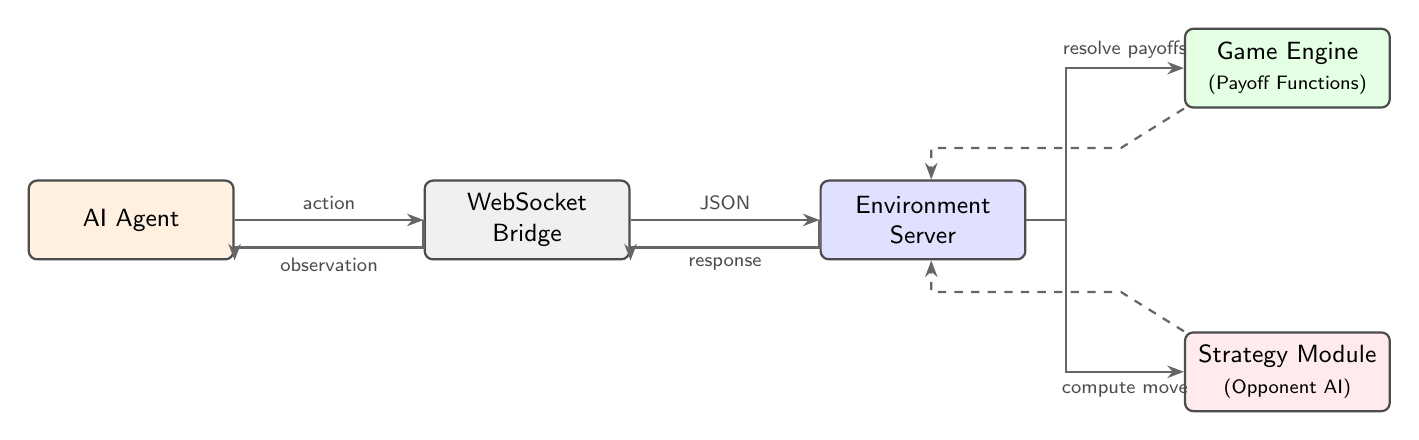
\begin{tikzpicture}[
    node distance=1.8cm and 2.4cm,
    box/.style={
        rectangle, draw=black!70, thick,
        fill=#1, minimum width=2.6cm, minimum height=1cm,
        font=\small\sffamily, align=center, rounded corners=3pt
    },
    box/.default={blue!8},
    arrow/.style={-{Stealth[length=6pt]}, thick, draw=black!60},
    lbl/.style={font=\scriptsize\sffamily, text=black!70}
]

% Agent node
\node[box=orange!12] (agent) {AI Agent};

% WebSocket bridge
\node[box=gray!12, right=of agent] (ws) {WebSocket\\Bridge};

% Environment server
\node[box=blue!12, right=of ws] (server) {Environment\\Server};

% Game engine
\node[box=green!10, above right=0.9cm and 2cm of server] (engine)
    {Game Engine\\{\scriptsize (Payoff Functions)}};

% Strategy module
\node[box=red!8, below right=0.9cm and 2cm of server] (strat)
    {Strategy Module\\{\scriptsize (Opponent AI)}};

% Arrows: agent <-> websocket <-> server
\draw[arrow] (agent.east) -- node[above, lbl] {action} (ws.west);
\draw[arrow] (ws.west) -- ++(0,-0.35) -| node[below, lbl, pos=0.25]
    {observation} (agent.south east);

\draw[arrow] (ws.east) -- node[above, lbl] {JSON} (server.west);
\draw[arrow] (server.west) -- ++(0,-0.35) -| node[below, lbl, pos=0.25]
    {response} (ws.south east);

% Arrows: server -> engine, server -> strategy
\draw[arrow] (server.east) -- ++(0.5,0) |- node[above, lbl, pos=0.75]
    {resolve payoffs} (engine.west);
\draw[arrow] (server.east) -- ++(0.5,0) |- node[below, lbl, pos=0.75]
    {compute move} (strat.west);

% Return arrows
\draw[arrow, dashed] (engine.south west) -- ++(-0.8,-0.5) -|
    ([xshift=3pt]server.north);
\draw[arrow, dashed] (strat.north west) -- ++(-0.8,0.5) -|
    ([xshift=3pt]server.south);

\end{tikzpicture}
}
\vspace{6pt}

{\small\color{WLegend}OpenEnv platform\;\;$\cdot$\;\;Gymnasium API\;\;$\cdot$\;\;
WebSocket\;\;$\cdot$\;\;FastAPI}
\end{frame}

% === 9: Governance ===
\begin{frame}{Meta-governance: agents change the rules during play}
\centering
\resizebox{0.90\textwidth}{!}{% governance_flow.tex -- TikZ diagram of governance proposal -> vote -> apply flow
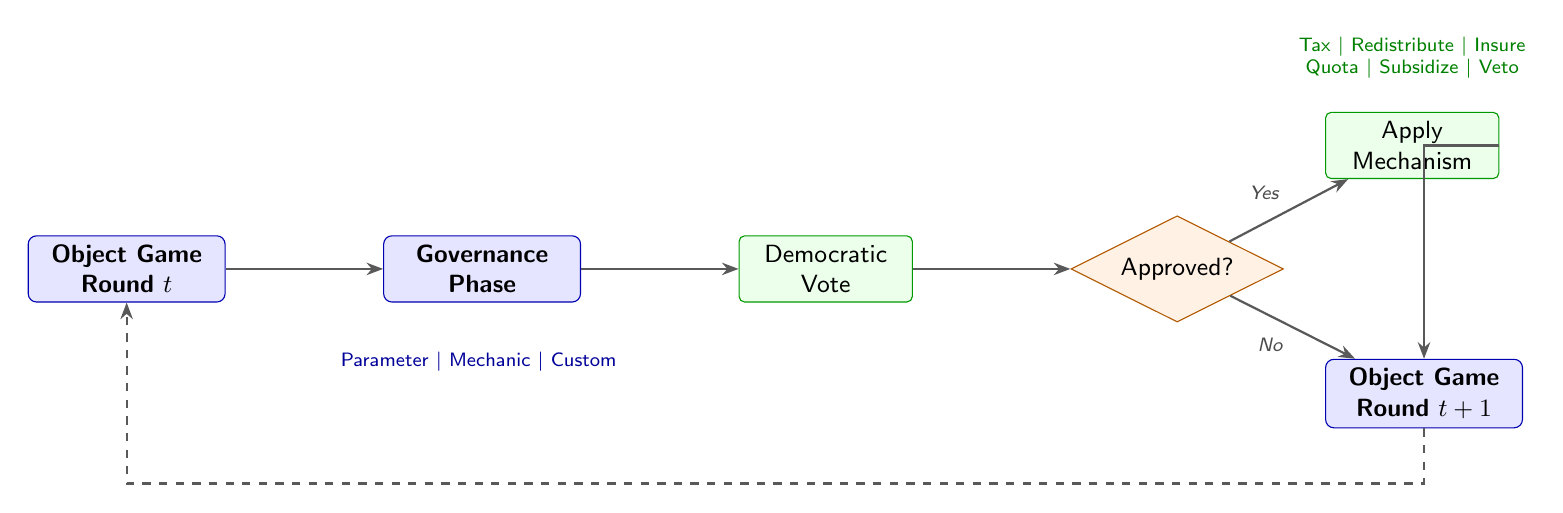
\begin{tikzpicture}[
    node distance=1.5cm and 2cm,
    phase/.style={rectangle, draw=blue!70!black, fill=blue!10,
        minimum width=2.5cm, minimum height=0.8cm, align=center,
        font=\small\bfseries, rounded corners=3pt},
    action/.style={rectangle, draw=green!60!black, fill=green!8,
        minimum width=2.2cm, minimum height=0.7cm, align=center,
        font=\small, rounded corners=2pt},
    decision/.style={diamond, draw=orange!70!black, fill=orange!10,
        minimum width=1.5cm, minimum height=1cm, align=center,
        font=\small, aspect=2},
    arrow/.style={-{Stealth[length=6pt]}, thick, draw=gray!70!black},
    label/.style={font=\scriptsize\itshape, text=gray!60!black}
]

% Main flow
\node[phase] (play) {Object Game\\Round $t$};
\node[phase, right=of play] (propose) {Governance\\Phase};
\node[action, right=of propose] (vote) {Democratic\\Vote};
\node[decision, right=of vote] (approve) {Approved?};
\node[action, above right=0.8cm and 1.2cm of approve] (apply) {Apply\\Mechanism};
\node[phase, below right=0.8cm and 1.2cm of approve] (next) {Object Game\\Round $t+1$};

% Arrows
\draw[arrow] (play) -- (propose);
\draw[arrow] (propose) -- (vote);
\draw[arrow] (vote) -- (approve);
\draw[arrow] (approve) -- node[label, above left] {Yes} (apply);
\draw[arrow] (approve) -- node[label, below left] {No} (next);
\draw[arrow] (apply) -| (next);

% Proposal types annotation
\node[below=0.5cm of propose, font=\scriptsize, align=center, text=blue!60!black] {
    Parameter $|$ Mechanic $|$ Custom
};

% Mechanism types annotation
\node[above=0.3cm of apply, font=\scriptsize, align=center, text=green!50!black] {
    Tax $|$ Redistribute $|$ Insure\\
    Quota $|$ Subsidize $|$ Veto
};

% Loop back arrow
\draw[arrow, dashed] (next.south) -- ++(0,-0.7) -| (play.south);

\end{tikzpicture}
}
\vspace{6pt}
\begin{columns}[T]
\column{0.44\textwidth}
\wcard[0.38\textwidth]{\textbf{\color{WAccent}Proposal types}\\[2pt]
{\small\color{WLegend}Parameter $\cdot$ Mechanic $\cdot$ Custom}}
\column{0.44\textwidth}
\wcard[0.38\textwidth]{\textbf{\color{WAccent}Mechanisms}\\[2pt]
{\small\color{WLegend}Tax, redistribute, insure, quota, veto}}
\end{columns}
\end{frame}

% === 10: Training pipeline ===
\begin{frame}{GRPO / DPO training pipeline}
\centering
\resizebox{0.88\textwidth}{!}{% training_pipeline.tex -- TikZ diagram of GRPO/DPO training loop
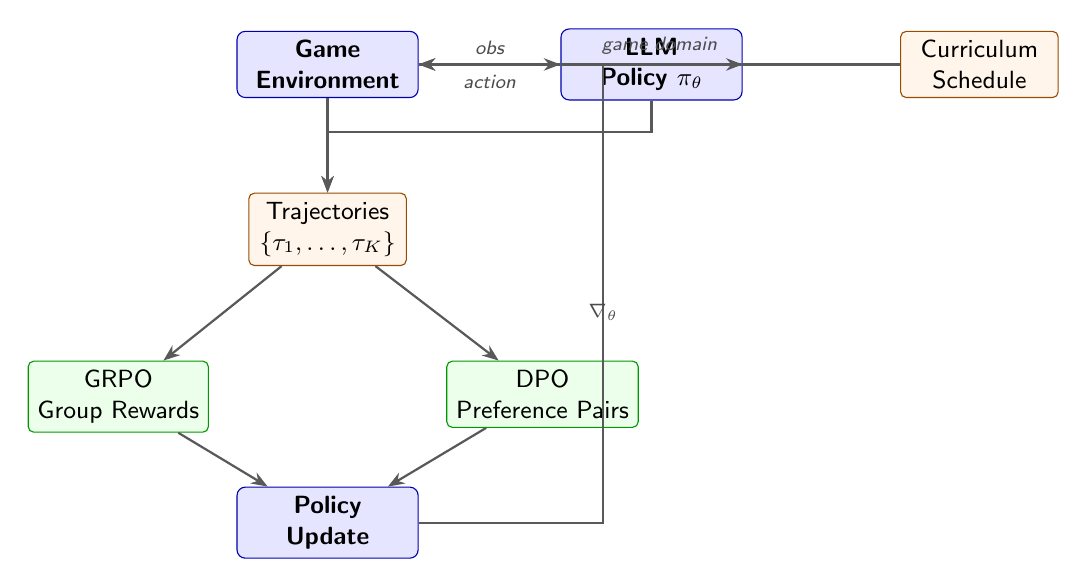
\begin{tikzpicture}[
    node distance=1.2cm and 1.8cm,
    component/.style={rectangle, draw=blue!70!black, fill=blue!10,
        minimum width=2.3cm, minimum height=0.8cm, align=center,
        font=\small\bfseries, rounded corners=3pt},
    process/.style={rectangle, draw=green!60!black, fill=green!8,
        minimum width=2.2cm, minimum height=0.7cm, align=center,
        font=\small, rounded corners=2pt},
    data/.style={rectangle, draw=orange!60!black, fill=orange!8,
        minimum width=2cm, minimum height=0.6cm, align=center,
        font=\small, rounded corners=2pt},
    arrow/.style={-{Stealth[length=6pt]}, thick, draw=gray!70!black},
    label/.style={font=\scriptsize\itshape, text=gray!60!black}
]

% Game environment
\node[component] (env) {Game\\Environment};
\node[component, right=of env] (policy) {LLM\\Policy $\pi_\theta$};

% Trajectory collection
\node[data, below=of env] (traj) {Trajectories\\$\{\tau_1, \ldots, \tau_K\}$};

% Two training paths
\node[process, below left=1.2cm and 0.5cm of traj] (grpo) {GRPO\\Group Rewards};
\node[process, below right=1.2cm and 0.5cm of traj] (dpo) {DPO\\Preference Pairs};

% Policy update
\node[component, below=2.8cm of traj] (update) {Policy\\Update};

% Curriculum
\node[data, right=2cm of policy] (curriculum) {Curriculum\\Schedule};

% Arrows
\draw[arrow] (env) -- (policy) node[midway, above, label] {obs};
\draw[arrow] (policy) -- (env) node[midway, below, label] {action};
\draw[arrow] (env) -- (traj);
\draw[arrow] (policy.south) -- ++(0,-0.4) -| (traj);
\draw[arrow] (traj) -- (grpo);
\draw[arrow] (traj) -- (dpo);
\draw[arrow] (grpo) -- (update);
\draw[arrow] (dpo) -- (update);
\draw[arrow] (update) -- ++(3.5,0) |- (policy.east) node[near start, below, label] {$\nabla_\theta$};
\draw[arrow] (curriculum) -- (env.east |- curriculum) node[midway, above, label] {game domain};

\end{tikzpicture}
}
\vspace{6pt}
\begin{columns}[T]
\column{0.44\textwidth}
\wcard[0.38\textwidth]{\textbf{\color{WAccent}GRPO}\\[2pt]
{\small\color{WLegend}Group relative rewards;\\compare within rollout group}}
\column{0.44\textwidth}
\wcard[0.38\textwidth]{\textbf{\color{WAccent}DPO}\\[2pt]
{\small\color{WLegend}Cooperative $\succ$ exploitative;\\no reward model needed}}
\end{columns}
\end{frame}

% === 11: Results ===
\begin{frame}{Tournament results}
\centering
\resizebox{0.78\textwidth}{!}{% tournament_heatmap.tex -- Illustrative cooperation-rate heatmap
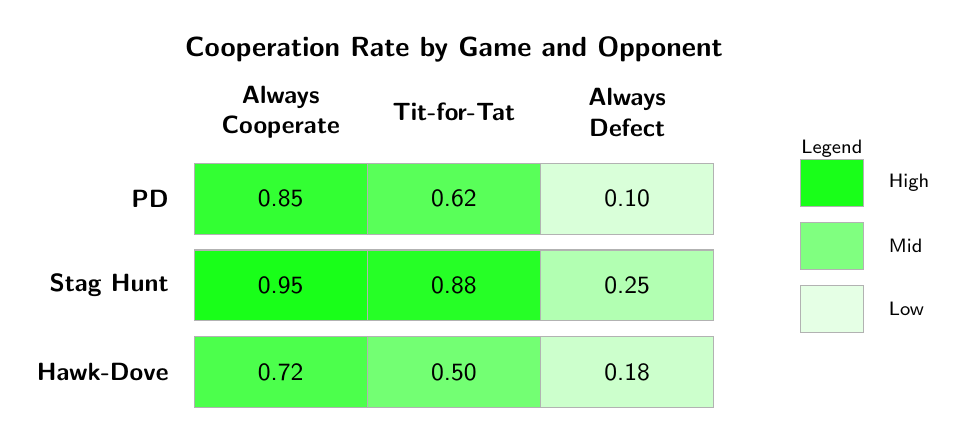
\begin{tikzpicture}[
    cell/.style={minimum width=2.2cm, minimum height=0.9cm,
                 font=\small, align=center},
    header/.style={font=\small\bfseries\sffamily, align=center},
    lbl/.style={font=\scriptsize\sffamily}
]

% Color helper: map a value in [0,1] to a green shade
\newcommand{\heatcell}[4]{%
    % #1=x, #2=y, #3=value (0-100), #4=display text
    \fill[green!#3!white] (#1-1.1, #2-0.45) rectangle (#1+1.1, #2+0.45);
    \draw[black!30] (#1-1.1, #2-0.45) rectangle (#1+1.1, #2+0.45);
    \node[cell] at (#1, #2) {#4};
}

% Title
\node[font=\sffamily\bfseries] at (4.4, 3.5)
    {Cooperation Rate by Game and Opponent};

% Column headers (strategies)
\node[header] at (2.2, 2.7) {Always\\Cooperate};
\node[header] at (4.4, 2.7) {Tit-for-Tat};
\node[header] at (6.6, 2.7) {Always\\Defect};

% Row headers (games)
\node[header, anchor=east] at (0.9, 1.6) {PD};
\node[header, anchor=east] at (0.9, 0.5) {Stag Hunt};
\node[header, anchor=east] at (0.9,-0.6) {Hawk-Dove};

% Row 1: Prisoner's Dilemma
\heatcell{2.2}{1.6}{80}{0.85}
\heatcell{4.4}{1.6}{65}{0.62}
\heatcell{6.6}{1.6}{15}{0.10}

% Row 2: Stag Hunt
\heatcell{2.2}{0.5}{90}{0.95}
\heatcell{4.4}{0.5}{85}{0.88}
\heatcell{6.6}{0.5}{30}{0.25}

% Row 3: Hawk-Dove
\heatcell{2.2}{-0.6}{70}{0.72}
\heatcell{4.4}{-0.6}{55}{0.50}
\heatcell{6.6}{-0.6}{20}{0.18}

% Color legend
\begin{scope}[shift={(8.8, 0.5)}]
    \node[lbl, anchor=south] at (0.4, 1.5) {Legend};
    \foreach \v/\y/\t in {90/1.0/High, 50/0.2/Mid, 10/-0.6/Low} {
        \fill[green!\v!white] (0, \y) rectangle (0.8, \y+0.6);
        \draw[black!30] (0, \y) rectangle (0.8, \y+0.6);
        \node[lbl, anchor=west] at (1.0, \y+0.3) {\t};
    }
\end{scope}

\end{tikzpicture}
}
\vspace{4pt}

{\small\color{WLegend}Illustrative data. Full multi-model results TBD.}
\end{frame}

% === 12: Close ===
\begin{frame}[plain]
\vfill
\begin{center}
{\fontsize{36}{40}\selectfont\color{WAccent}\bfseries Kant}\\[10pt]
{\color{WLegend}Game theory as an alignment substrate.}\\[24pt]
{\small\color{WLegend}\texttt{github.com/wisent-ai/OpenEnv}\\[4pt]
\texttt{wisent.ai}}
\end{center}
\vfill
\end{frame}

\end{document}
